\documentclass[11pt]{article}
\renewcommand{\familydefault}{\sfdefault}

% Make margins smaller
\usepackage[top=0.9in, bottom=0.9in, left=1in, right=1in]{geometry}
% more advanced mathematical symbols
\usepackage{amsfonts}
\usepackage{amssymb}
\usepackage{amsmath}
\usepackage{bm}
\usepackage{bold-extra} % bold texttt
\usepackage{graphicx}
\usepackage{enumerate}
\usepackage[font=small,labelfont=bf]{caption} % Required for specifying captions to tables and figures
\usepackage{pgfgantt} % gantt chart!
\usepackage{titling}
\usepackage{gensymb}
\usepackage{setspace}
\renewcommand{\baselinestretch}{1.2} 

\graphicspath{ {./images/} }

% so that we can skip any number of items in an enumeration
\makeatletter
\newcommand{\skipitems}[1]{%
  \addtocounter{\@enumctr}{#1}%
}
\makeatother

\begin{document}

\title{\textbf{Virtual Reality Summative}}
\date{for 15th March 2019}
\author{Bradley Mackey}
\maketitle


\section*{Question Remarks}

\begin{enumerate}
\item 
\texttt{get\_raw\_imu\_data()} returns the raw data readings from the \texttt{.csv} file (given that it is located in the same directory), returning a 2D array of data rows.\\
\texttt{sanitize\_imu\_data(data)} cleans the data as specified, returning a 2D array of rows of the modified data.\\
\texttt{euler\_to\_qtrn(euler)} computes a quaternion $(a,b,c,d)$ from a given array of Euler angles $(\theta,\psi,\phi)$, the rotations around the $x$-, $y$- and $z$-axes respectively.\\
\texttt{qtrn\_to\_euler(qtrn)} computes the Euler angles $(\theta,\psi,\phi)$ for a given quaternion representation $(a,b,c,d)$.\\
\texttt{qtrn\_conj(qtrn)} takes a quaternion $(a,b,c,d)$ and returns its conjugate, $(a,-b,-c,-d)$.\\
\texttt{qtrn\_mult(qtrn\_1, qtrn\_2)} computes the product of 2 quaternions, returning this product $(a,b,c,d)$.

% NO REPORT REQUIRED FOR QUESTION #2
\skipitems{1} 

% QUESTION 3: Try a few different alpha values (e.g., 0.01, 0.1, ...), investigate and comment on their effect on drift compensation in your report (7 marks)

\item 

For tilt correction, we adjust the $z$ `up' vector to align with the true up vector in the real world, as measured by the accelerometer. This is because this is the first angle measured by the IMU, so we assume this is up. This could well be the case if the IMU is physically mounted in such a way that the $z$ vector points upright.
For the smallest values of $\alpha_{tilt}$ ($<0.001$), very little drift correction is applied, making the effect of this similar to no drift correction at all, as can bee seen in the dead-reckoning.
The effect of this would remain a smooth experience for a user of the VR headset, but the drift problem has not been addressed, and a clear drift of around $20\degree$ can be see at the end of the capture.
For very large values of $\alpha_{tilt}$ (0.1--1), extremely erratic and sharply-changing angles can be seen in the $\phi$ and $\psi$ Euler angles as the tilt correction is applied. 
These rapid angle changes are due to the fact that as a large amount of tilt correction is applied with each reading, the angle must be sharply adjusted.
This would make for an unusable and very unpleasant experience for a VR user, as the world frame would constantly `judder' back into a correct orientation despite the user's head movements---expect nausea!

I found that an $\alpha_{tilt}$ value of around 0.001 resulted in good drift correction, able to dramatically reduce the amount of drift present at the end of the dead-reckoning reading. This is visible in Figure \ref{fig:euler-angles}.
A reduction in correction noise could be applied by taking the average position of the `up vector' over a number of samples in proximity, meaning that successive corrections are changed by a similar angle, making angle changes less sharp and noticable.

% QUESTION 4: Try a few different alpha values (e.g., 0.01, 0.1, ...), investigate and comment on their effect on drift compensation in your report (5 marks).

\item 
Yaw correction effects the Euler angle around the $z$-axis ($\psi$ angle) because of the initial mounted positioning of the IMU, explained above.
Firstly, I found that the yaw correction had a much smaller effect than compared to tilt correction, due to the tilt correction already having a large positive effect on reducing the drift of the readings. 

Keeping $\alpha_{tilt}$ set at 0.001, I found that all values of $\alpha_{yaw}$ greater than 0.00001 were able to correct additional minor amounts of drift about the $z$-axis, values below this being unnoticable.  
Similarly to tilt correction, I found values of $\alpha_{yaw}$ that were larger than $\alpha_{tilt}$ caused conflicts in the drift correction, and resulted in incorrect readings being produced. This would also have the effect of causing very juddery motion for the viewer of the VR world.

In the end, this left only one real effective value for $\alpha_{yaw}$, 0.0001. This was able to correct slight drift around the $z$-axis and allow the drift at the end of the reading to end up very close to zero.

\end{enumerate}

\section*{Visualisations}

\begin{figure}[htp]

\centering
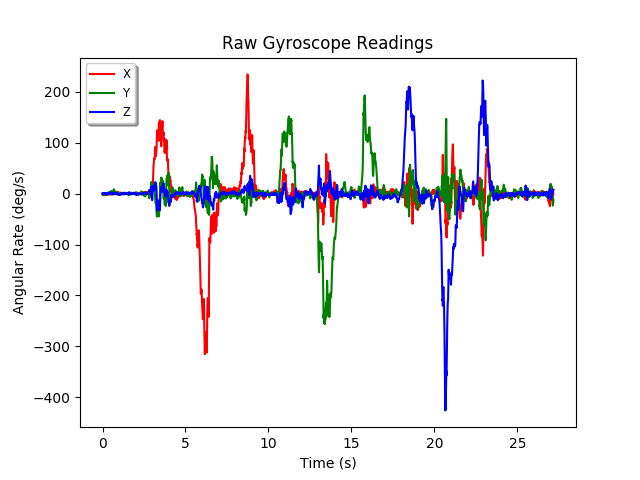
\includegraphics[width=.32\textwidth]{gyro-unaltered}\hfill
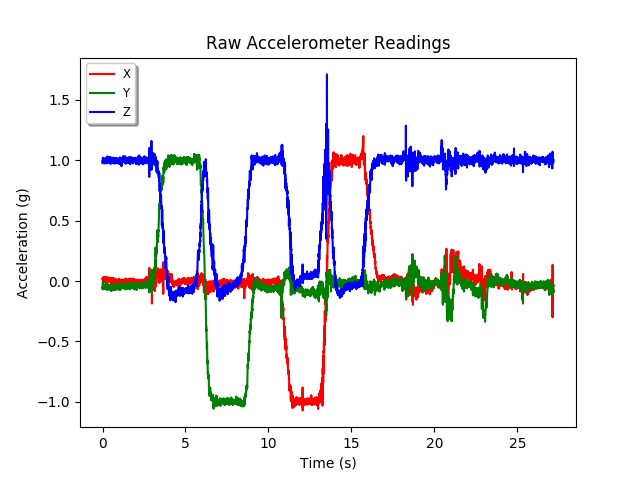
\includegraphics[width=.32\textwidth]{acc-unaltered}\hfill
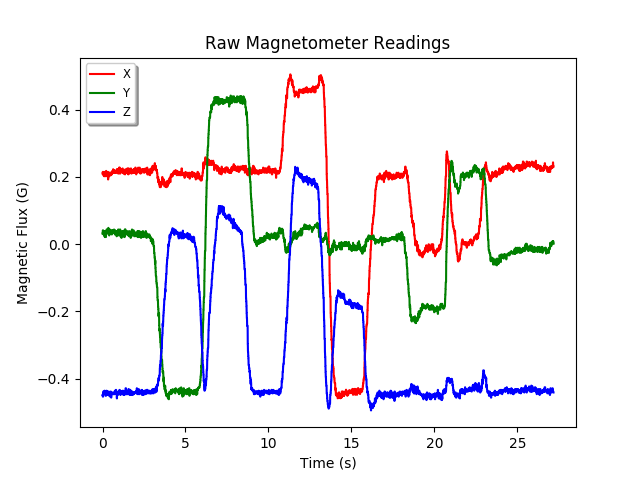
\includegraphics[width=.32\textwidth]{mag-unaltered}

\caption{Raw sensor readings from the IMU. Raw accelerometer data (centre) clearly displaying the $z$-axis as the initial `up' position (reading of $g$), so tilt corrections are made towards this axis, yaw corrections are made around this axis.}
\label{fig:raw-readings}

\end{figure}

\begin{figure}[htp]

\centering
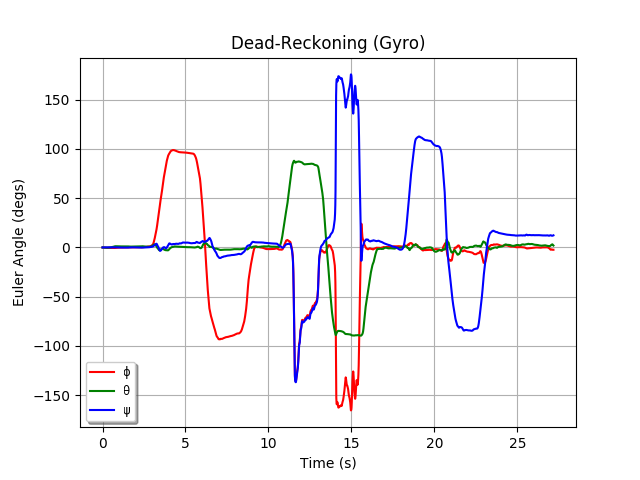
\includegraphics[width=.32\textwidth]{1gyro_dead}\hfill
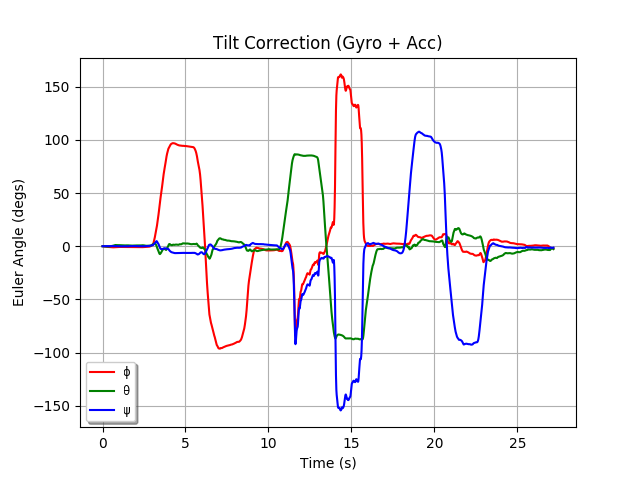
\includegraphics[width=.32\textwidth]{2gyro_acc}\hfill
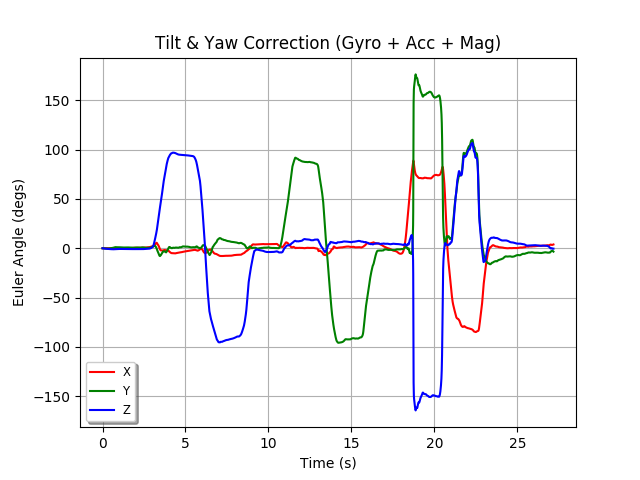
\includegraphics[width=.32\textwidth]{3gyro_acc_mag}

\caption{Euler angle readings, with and without various levels of correction. For tilt correction, $\alpha_{tilt}=0.001$. For tilt \& yaw correction, $\alpha_{tilt}=0.001$, $\alpha_{yaw}=0.0001$. Notice the clear improvements and reduction in axis drift as more levels of error correction are added to the raw dead-reckoning data. Error reduction can be most clearly seen at the end of the reading, where the drift is minimal with corrections. The erratic angle changes occurring at $t\approx14$ and $t\approx15$ is caused by gimbal lock induced by the rotation of the IMU and the fact we are displaying this data as Euler angles, which is a major limitation of the Euler angle representation.}
\label{fig:euler-angles}

\end{figure}

\begin{figure}[htp]

\centering
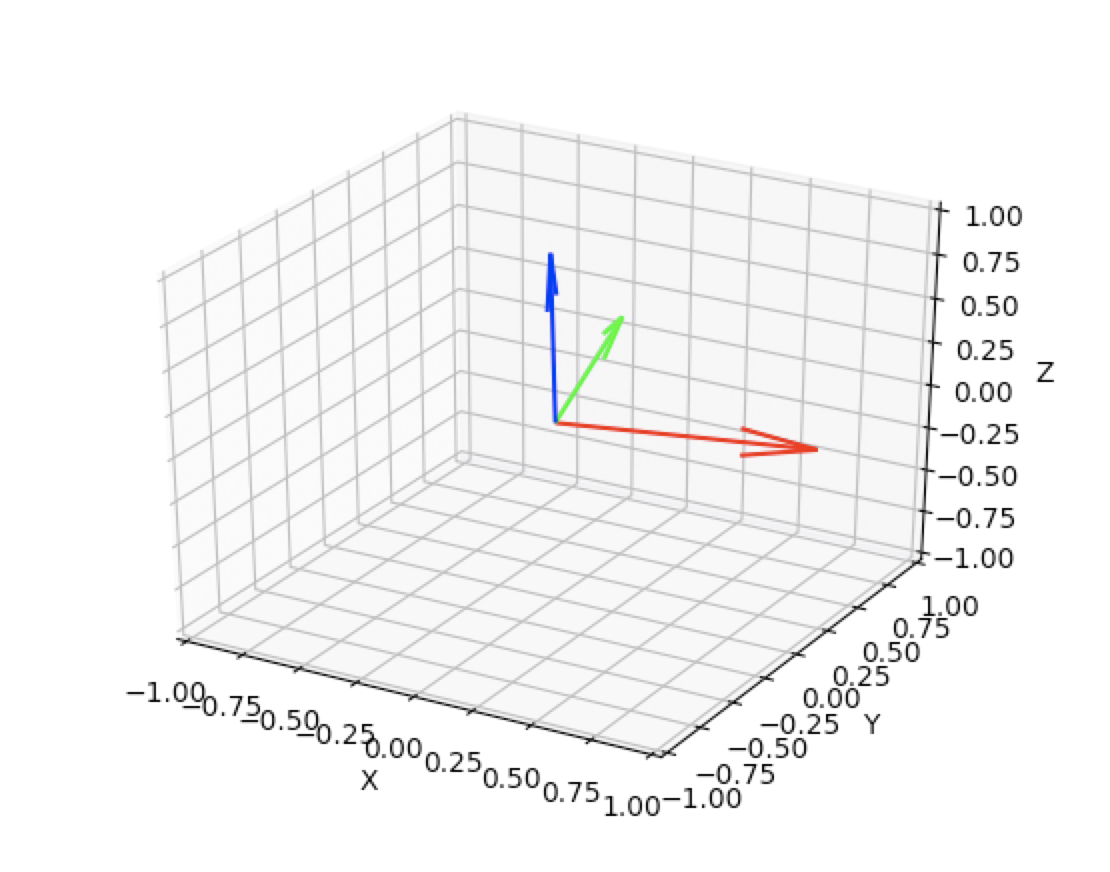
\includegraphics[width=.32\textwidth]{4gyro_after}\hfill
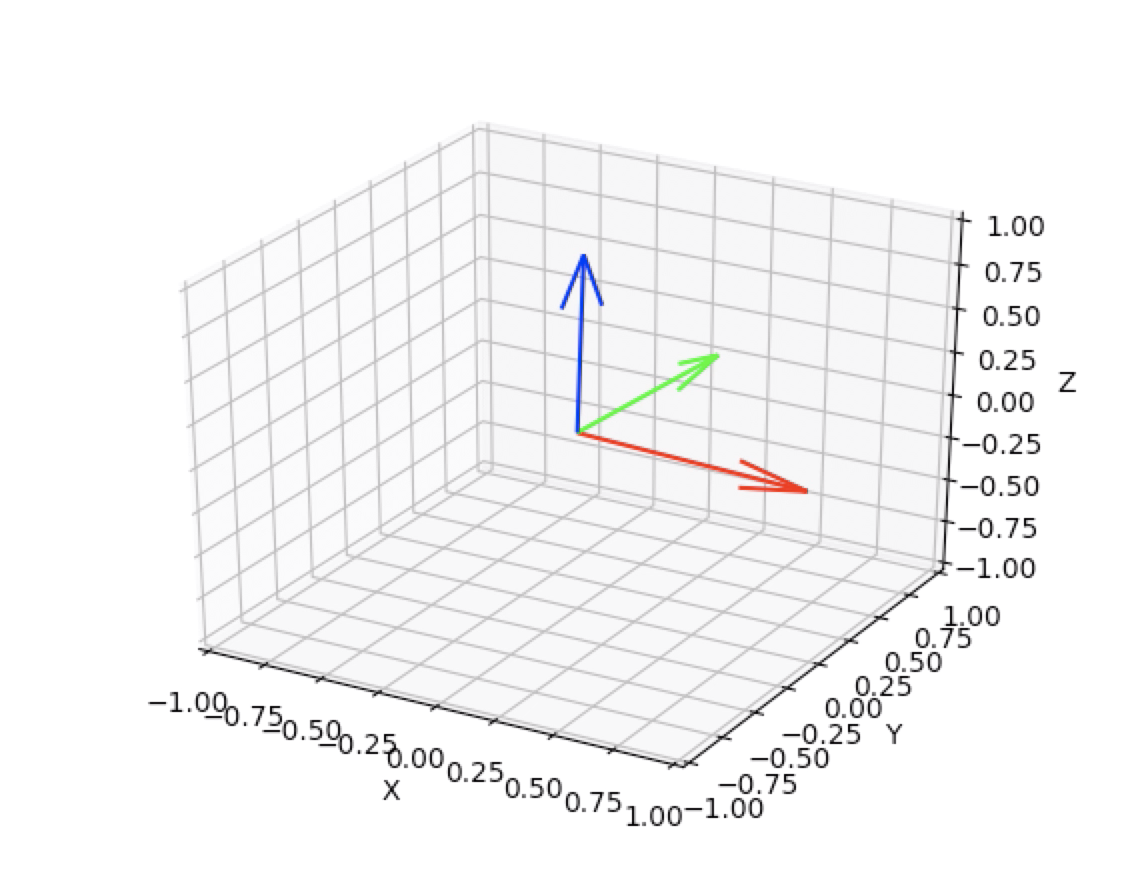
\includegraphics[width=.32\textwidth]{5acc_after}\hfill
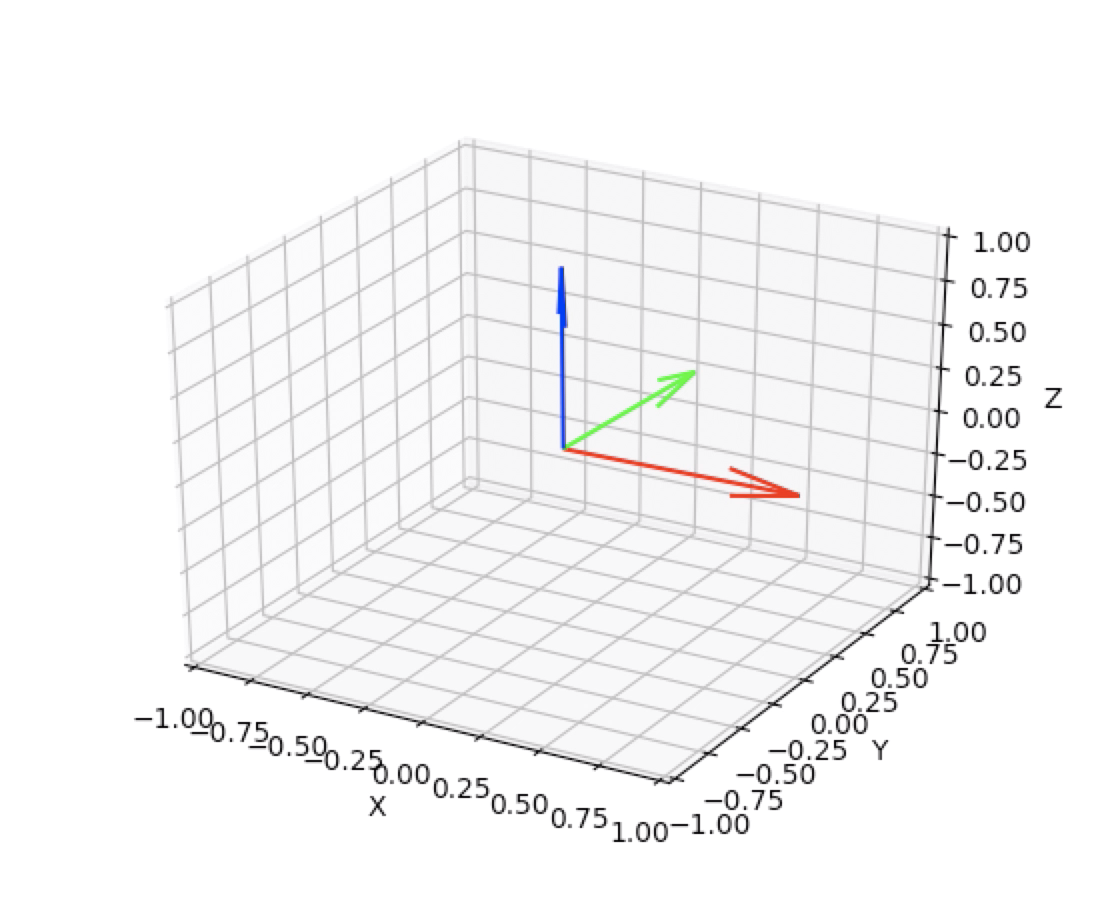
\includegraphics[width=.32\textwidth]{6mag_after}

\caption{From left to right: dead reckoning, tilt correction, tilt \& yaw correction. The blue, green and red vectors correspond to the $z$, $y$ and $x$ vectors respectively. Vectors shown are the final positions of the IMU after all data points were played back. See document prose for more information.}
\label{fig:3d}

\end{figure}

Figure \ref{fig:3d} shows screenshots from the playback of data for each correction method. It is clear there is less drift as more levels of correction are included in the calculation of the true orientation Data was recorded for each of the correction methods and interactively displayed in 3D using \texttt{matplotlib} for Python. 

Due to technological constraints, data was recorded at 40x slower than realtime, recorded and played back at realtime, then half speed (the rendering was very slow on my computer for some reason). With all levels of correction, the micro-judders caused by twitchy movements of the IMU are not able to be corrected, so these slight judders are visible in all animations. In the case of the corrected movements, the judders are somewhat exaggerated at some points at the corrections are applied to the rotation, but this effect is quite minor. The reduced drift is noticeable in both the tilt and tilt \& yaw corrected movements though---although the difference between these two is very small. 

Overall, I found that tilt correction alone was able to dramatically increase the positional accuracy of the raw IMU data, yaw correction only slightly improving this accuracy.


\end{document}